\documentclass[11pt]{beamer}

%%%%%%%%%%%%%%%%
% Packages
%%%%%%%%%%%%%%%%
\usepackage{booktabs}
\usepackage{hyperref}		% produces hyperlinks
\usepackage{multirow}	% allows for rows that span multiple rows in tables

%%%%%%%%%%%%%%%%
% Prelims
%%%%%%%%%%%%%%%%

\usetheme[titleformat=smallcaps, progressbar=frametitle]{metropolis}
\author{Sergio I. Garcia-Rios}
\title{Introduction to the Course}
\institute{Government 3990: Statistics in the Social Science}
\date{}




\begin{document}
\maketitle

%%%%%%%%%%%%%%%%%%%%%%%%%%%%%%%%%%%

\section{General info}

%%%%%%%%%%%%%%%%%%%%%%%%%%%%%%%%%%%

\begin{frame}
\frametitle{Teaching team}

\begin{itemize}

\item Professor: Sergio Garcia-Rios \url{garcia.rios@cornell.edu}


\end{itemize}

\end{frame}

%%%%%%%%%%%%%%%%%%%%%%%%%%%%%%%%%%%

\begin{frame}
\frametitle{Required materials}

\begin{itemize}

\item OpenIntro Statistics, 4th Edition: \url{http://openintro.org/os}

\begin{itemize}
\item The textbook is freely available online. You're encouraged to read on screen but you can print it out. If you prefer a paperback version you can buy it at the cost of printing (around \$20) on Amazon
\end{itemize}

\item (optional) Calculator (just something that can do square roots)

\end{itemize}

\end{frame}

%%%%%%%%%%%%%%%%%%%%%%%%%%%%%%%%%%%

\begin{frame}
\frametitle{Webpage}


\centering
{\Large Puzzle Solving with Data - GOVT 3990
\url{garciarios.github.io/govt_3990} 
}

\end{frame}

%%%%%%%%%%%%%%%%%%%%%%%%%%%%%%%%%%

\section{Course structure}

%%%%%%%%%%%%%%%%%%%%%%%%%%%%%%%%%%

\begin{frame}[shrink]
\frametitle{Learning units and course outline}

\begin{itemize}

\item Pictures and summaries of data
\begin{itemize}
\item \alert{Unit 1 - Intro to data:} Observational studies \& non-causal inference, 
principles of experimental design \& causal inference, exploratory data analysis, 
introduction to simulation-based statistical inference.
\end{itemize}

\item Mathematics behind statistics
\begin{itemize}
\item \alert{Unit 2 - Probability \& distributions:} Basics of probability and chance 
processes, Bayesian perspective in statistical inference, the normal and binomial 
distributions.
\end{itemize}

\item Statistical inference
\begin{itemize}
\item \alert{Unit 3 - Framework for inference:} CLT, sampling distributions, and 
introduction to theoretical inference.
\item Midterm 1
\item \alert{Unit 4 - Statistical inference for numerical variables}
\item \alert{Unit 5 - Statistical inference for categorical variables}
\item Midterm 2
\end{itemize}

\item Modeling
\begin{itemize}
\item \alert{Unit 6 - Simple linear regression:} Bivariate correlation and causality, 
introduction to modeling.
\item \alert{Unit 7 - Multiple linear regression:} More advanced modeling with multiple 
predictors.
\item Final Exam
\end{itemize}

\end{itemize}

\end{frame}

%%%%%%%%%%%%%%%%%%%%%%%%%%%%%%%%%%

\begin{frame}
\frametitle{Course structure}

\begin{itemize}[<alert@+>]
\item Set of learning objectives and required and suggested readings for each unit.
\item Prior to beginning the unit complete the readings and familiarize yourselves with the learning objectives. \pause
\item Begin a new unit with a readiness assessment: individual or team. \pause
\item Class time: split between lecture, discussion/application, and lab. \pause
\item Complement your learning with problem sets. \pause
%\item Wrap up a unit with a performance assessment. 
\end{itemize}

\end{frame}

%%%%%%%%%%%%%%%%%%%%%%%%%%%%%%%%%%%
%
%\begin{frame}
%\frametitle{Teams}
%
%\begin{itemize}
%\item Highly functional teams of learners based on survey and pre-test.
%
%\item Team members first point of contact.
%
%\item Application exercises, labs, team readiness assessments, project.
%
%\item Study together, but anything that is not explicitly a team assignment must be 
%your own work.
%
%\item Peer evaluations to ensure that all team members contribute to the success of 
%the group and to address any potential issues early on.
%\begin{itemize}
%\item If you feel that there are issues within your team, you are encouraged to 
%discuss it with your team members and to bring it to my or your TA's attention ASAP (
%don't wait till things get worse).
%\end{itemize}
%
%\end{itemize}
%
%\end{frame}
%
%%%%%%%%%%%%%%%%%%%%%%%%%%%%%%%%%%%
%
%\begin{frame}
%\frametitle{Clickers}
%
%\alert{\textbf{Objective:}} Two-way communication and instant feedback.
%
%\begin{itemize}
%\item Readiness assessments (graded for accuracy)
%
%\item Questions throughout lecture (graded for participation)
%\begin{itemize}
%\item Get credit for the day you by responding to at least 75\% of the questions.
%\item Up to three unexcused late arrivals or absences.
%\end{itemize}
%
%\item Register your clicker at \url{https://www1.iclicker.com/register-clicker} 
%(Student ID = Net ID)
%\begin{itemize}
%\item If you bought a used clicker, the registration process might ask for a payment. 
%You don't need to pay, you'll be able to register in class.
%\end{itemize}
%
%\end{itemize}
%
%\end{frame}
%\end{document}
%%%%%%%%%%%%%%%%%%%%%%%%%%%%%%%%%%%

\begin{frame}
\frametitle{Project}

\alert{\textbf{Objective:}} Give you independent applied research experience using real data and 
statistical methods.

\begin{itemize}

\item Proposal and presentation: due mid-semester

\item Final Presentation: last week of semester


\end{itemize}

\end{frame}




%%%%%%%%%%%%%%%%%%%%%%%%%%%%%%%%%%

\begin{frame}
\frametitle{Exams}

%\begin{center}
%%\rowcolor{1}{}{gray}
%%\renewcommand\arraystretch{1.25}
%{\footnotesize
%\begin{tabular}{ r | l }
%Midterm 1								& Feb 12 \\    
%Midterm 2 							& Feb 12 \\    
%Final 								 & Feb 12   
%\end{tabular}
%}
%\end{center}


There will be one midterm.
\begin{itemize}
\item See course info for dates and times of the exams. 
\item Exam dates cannot be changed and no make-up exams will be given.
\item Calculator + cheat sheet allowed

\end{itemize}

\end{frame}


%%%%%%%%%%%%%%%%%%%%%%%%%%%%%%%%%%


\begin{frame}
\frametitle{Office Hours}
Visit the website if you need to schedule office hours
\begin{itemize}
\item At least 24 hrs in advance
\item Please choose only one slot, if you need more time, email me first 
\item If you schedule office hours, please do show up 
\end{itemize}
\end{frame}

%%%%%%%%%%%%%%%%%%%%%%%%%%%%%%%%%%

\begin{frame}
\frametitle{Students with disabilities}

Students with disabilities who believe they may need accommodations in this class are 
encouraged to contact the \alert{\href{https://www.sce.cornell.edu/sc/apply/disabilities.php}{Student with Disability 
Services Office}} telephone 607.254.4545; \url{e-mail sds_cu@cornell.edu} as soon as possible to better ensure that such 
accommodations can be made.


\end{frame}

%%%%%%%%%%%%%%%%%%%%%%%%%%%%%%%%%%

\section{Academic Dishonesty}

%%%%%%%%%%%%%%%%%%%%%%%%%%%%%%%%%%

\begin{frame}
\frametitle{Academic Dishonesty}

Any form of academic dishonesty will result in an immediate 0 on the given assignment 
and will be reported to the Office of Academic Integrity. Additional penalties may also 
be assessed if deemed appropriate. If you have any questions about whether something 
is or is not allowed, ask me beforehand.



\end{frame}


%%%%%%%%%%%%%%%%%%%%%%%%%%%%%%%%%%%

\section{Tips for success}

%%%%%%%%%%%%%%%%%%%%%%%%%%%%%%%%%%%

\begin{frame}
\frametitle{Tips for success}

{\footnotesize
\begin{itemize}[<alert@+>]
\item Complete the reading before a new unit begins, and then review again after the 
unit is over. \pause
\item Be an active participant during lectures and labs. \pause
\item Ask questions - during class or office hours, or by email. Ask me, and 
your classmates. \pause
\item Do the problem sets - start early and make sure you attempt and understand all 
questions. \pause

\item Start your project early and and allow adequate time to complete them. \pause
\item Give yourself plenty of time time to prepare a good cheat sheet for exams. This 
requires going through the material and taking the time to review the concepts that 
you're not comfortable with. \pause
\item Do not procrastinate - don't let a unit go by with unanswered questions as it 
will just make the following unit's material even more difficult to follow. 
\end{itemize}
}

\end{frame}


%%%%%%%%%%%%%%%%%%%%%%%%%%%%%%%%%%%

\section{To do}

%%%%%%%%%%%%%%%%%%%%%%%%%%%%%%%%%%%

\begin{frame}{To do}

\begin{itemize}

\item Download or purchase the textbook
\begin{itemize}
\item Download: \url{http://openintro.org/os}
\item Purchase: \url{http://openintro.org/os/amazon}
\end{itemize}

\item Go to the \alert{\href{https://garciarios.github.io/govt_3990/}{course website}}, read the syllabus, let me know if you have any questions.

\item Get started with your labs
\begin{itemize}
\item Lab 0 is due today
\end{itemize}

\end{itemize}

\end{frame}


%%%%%%%%%%%%%%%%%%%%%%%%%%%%%%%%%%%

\section{Let's get familiar with the website}

\section{An Example on the importance of (Good) Data Analysis and Presentation}


\begin{frame}{The \textit{Challenger} launch decision}
\begin{columns}
\begin{column}{0.5\textwidth}
In 1986, the Challenger space shuttle exploded moments after liftoff

Decision to launch one other most scrutinized in history

Failure of O-rings in the solid-fuel rocket boosters blamed for explosion

Could this failure have been foreseen? 
\end{column}
\begin{column}{0.5\textwidth}
\begin{center}
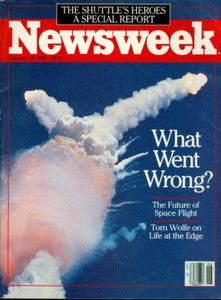
\includegraphics[scale=.5]{shuttle.jpg}
\end{center}
\end{column}
\end{columns}
\end{frame}


%%%%%%%%%%%%%%%%%%%%%%%%%%%%%%%%%%%
\begin{frame}{The \textit{Challenger} launch decision}
Morton-Thiokol engineers made this table \& worried about launching below 53 degrees (Why?)

\begin{scriptsize}
\begin{center}
\begin{tabular}{cc}
\toprule
\multicolumn{2}{c}{Flights with O-ring damage}\\
Flt Number      &       Temp (F)        \\
\midrule
2       &       70      \\
41b     &       57      \\
41c     &       63      \\
41d     &       70      \\
51c     &       53      \\
61a     &       79      \\
61c     &       58      \\
\bottomrule
\end{tabular}
\end{center}
\end{scriptsize}


\only<2>{\alert{O-ring would erode or have ``blow-by'' (2 ways to fail) in cold temp}}
\only<3>{\alert{Failed to convince administrators there was a danger}}
\only<4>{\alert{(Counter-argument:  ``damages at low and high temps'')}}
\only<5>{\alert{Are there problems with this presentation?  with the use of data?}}

\end{frame}
%%%%%%%%%%%%%%%%%%%%%%%%%%%%%%%%%%%

\begin{frame}{The \textit{Challenger} launch decision}
\begin{small}


Engineers did not consider successes, only failures; \\
selection on the dependent variable \pause

\begin{scriptsize}
\begin{center}
\begin{tabular}{ccccc}
\toprule
\multicolumn{5}{c}{All flights, chronological order}\\
Damage? &       Temp (F)        &      \quad \quad \quad        &       Damage? &       Temp (F)        \\
\midrule
No      &       66      &               &       No      &       78      \\
\color{red}\textbf{Yes}    &     \color{red}  70      &               &       No      &       67      \\
No      &       69      &               &     \color{red}   \textbf{Yes}    & \color{red}       53      \\
No      &       68      &               &       No      &       67      \\
No      &       67      &               &       No      &       75      \\
No      &       72      &               &       No      &       70      \\
No      &       73      &               &       No      &       81      \\
No      &       70      &               &       No      &       76      \\
\color{red} \textbf{Yes}    &   \color{red}     57      &               &       \color{red} \textbf{Yes}    &   \color{red}     79      \\
\color{red} \textbf{Yes}    &   \color{red}     63      &               &       No      &       76      \\
\color{red} \textbf{Yes}    &   \color{red}     70      &               &       \color{red} \textbf{Yes}    &   \color{red}     58      \\
\bottomrule
\end{tabular}
\end{center}
\end{scriptsize}
Other problems?  \pause Why sort by launch number?

\end{small}
\end{frame}
%%%%%%%%%%%%%%%%%%%%%%%%%%%%%%%%%%%

\begin{frame}{The \textit{Challenger} launch decision}
\begin{small}
\begin{scriptsize}
\begin{center}
\begin{tabular}{ccccc}
\toprule
\multicolumn{5}{c}{O-ring damage pre-Challenger, by temperature at launch}\\
Damage? &       Temp (F)        &       &       Damage? &       Temp (F)        \\
\midrule
\color{red} \textbf{Yes}        &       \color{red} 53  & \quad\quad\quad& \color{red} \textbf{Yes}     &       \color{red}70   \\
\color{red} \textbf{Yes}        &       \color{red}57   &       &       No       &       70      \\
\color{red} \textbf{Yes}        &       \color{red}58   &       &       No       &       70      \\
\color{red} \textbf{Yes}        &       \color{red}63   &       &       No       &       72      \\
No       &       66      &       &       No       &       73      \\
No       &       67      &       &       No       &       75      \\
No       &       67      &       &       No       &       76      \\
No       &       67      &       &       No       &       76      \\
No       &       68      &       &       No       &       78      \\
No       &       69      &       &       \color{red} \textbf{Yes}        &       \color{red}79   \\
\color{red} \textbf{Yes}        &       \color{red}70   &       &       No       &       81      \\
\bottomrule
\end{tabular}
\end{center}
\end{scriptsize} \pause
The evidence begins to speak for itself. \pause

What if engineers had made this table before the launch?

\end{small}
\end{frame}

%%%%%%%%%%%%%%%%%%%%%%%%%%%%%%%%%%%

\begin{frame} {The \emph{Challenger} launch decision}

Why didn't NASA make the right decision? \pause

Many answers in the literature:  \\
bureaucratic politics; group think; bounded rationality, etc \pause

But Edward Tufte thinks it may have been a matter of presentation \& modeling: \pause

\begin{itemize}
\item Never made the right tables or graphics

\item Selected only failure data

\item Never considered a simple statistical model
\end{itemize}
What do you think?  How would you approach the data?

\end{frame}

%%%%%%%%%%%%%%%%%%%%%%%%%%%%%%%%%%%

\begin{frame}{The \textit{Challenger} launch decision}

\small{How about a scatterplot?  Better for seeing relationships than a table. 

Vertical axis is an O-ring damage index (due to Tufte, who made the plot)} \pause

\begin{center}
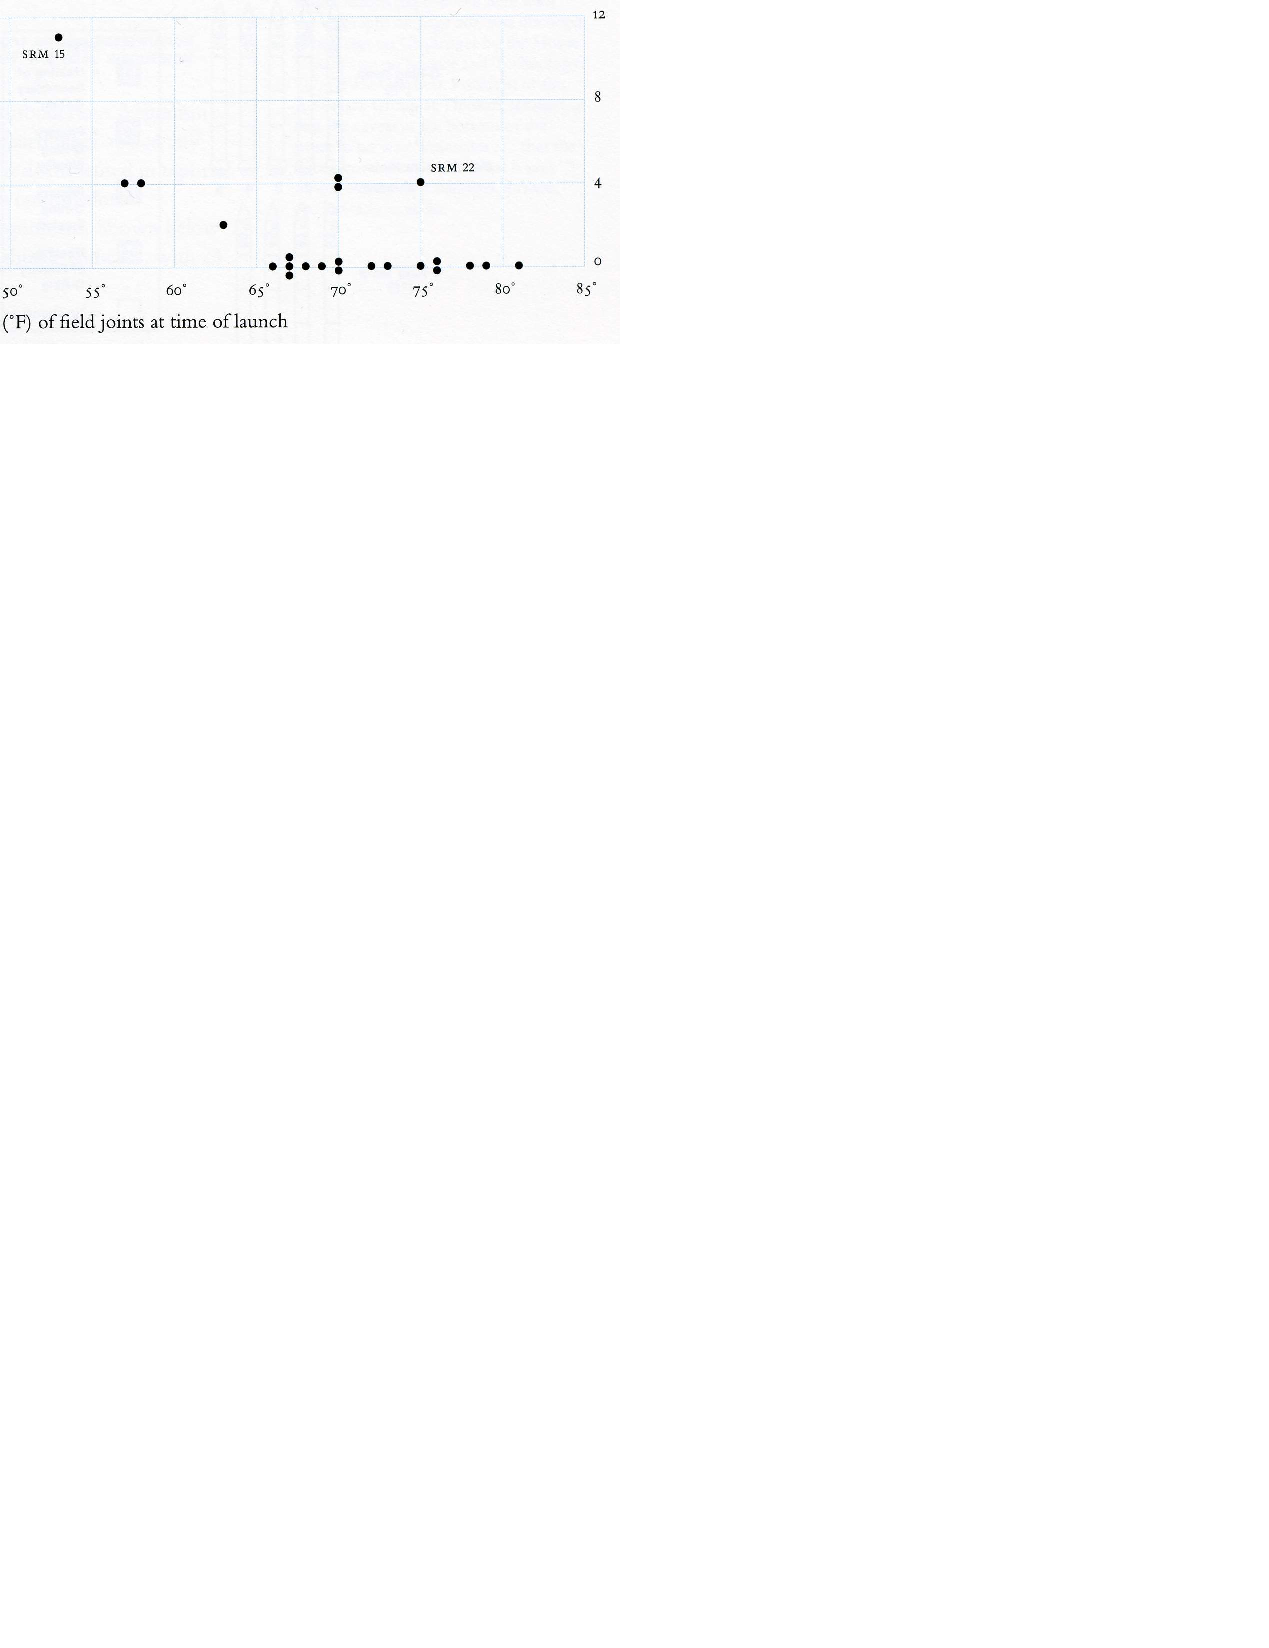
\includegraphics[scale= 0.68]{tufte_challenger_1}
\end{center}


Suspicious. \pause  What was the forecast temperature for launch?  
\end{frame}

%%%%%%%%%%%%%%%%%%%%%%%%%%%%%%%%%%%

\begin{frame}{The\emph{Challenger} launch decision}

What was the forecast temperature for launch? \pause 26  to 29 $^{\circ}$F! \pause

\begin{center}
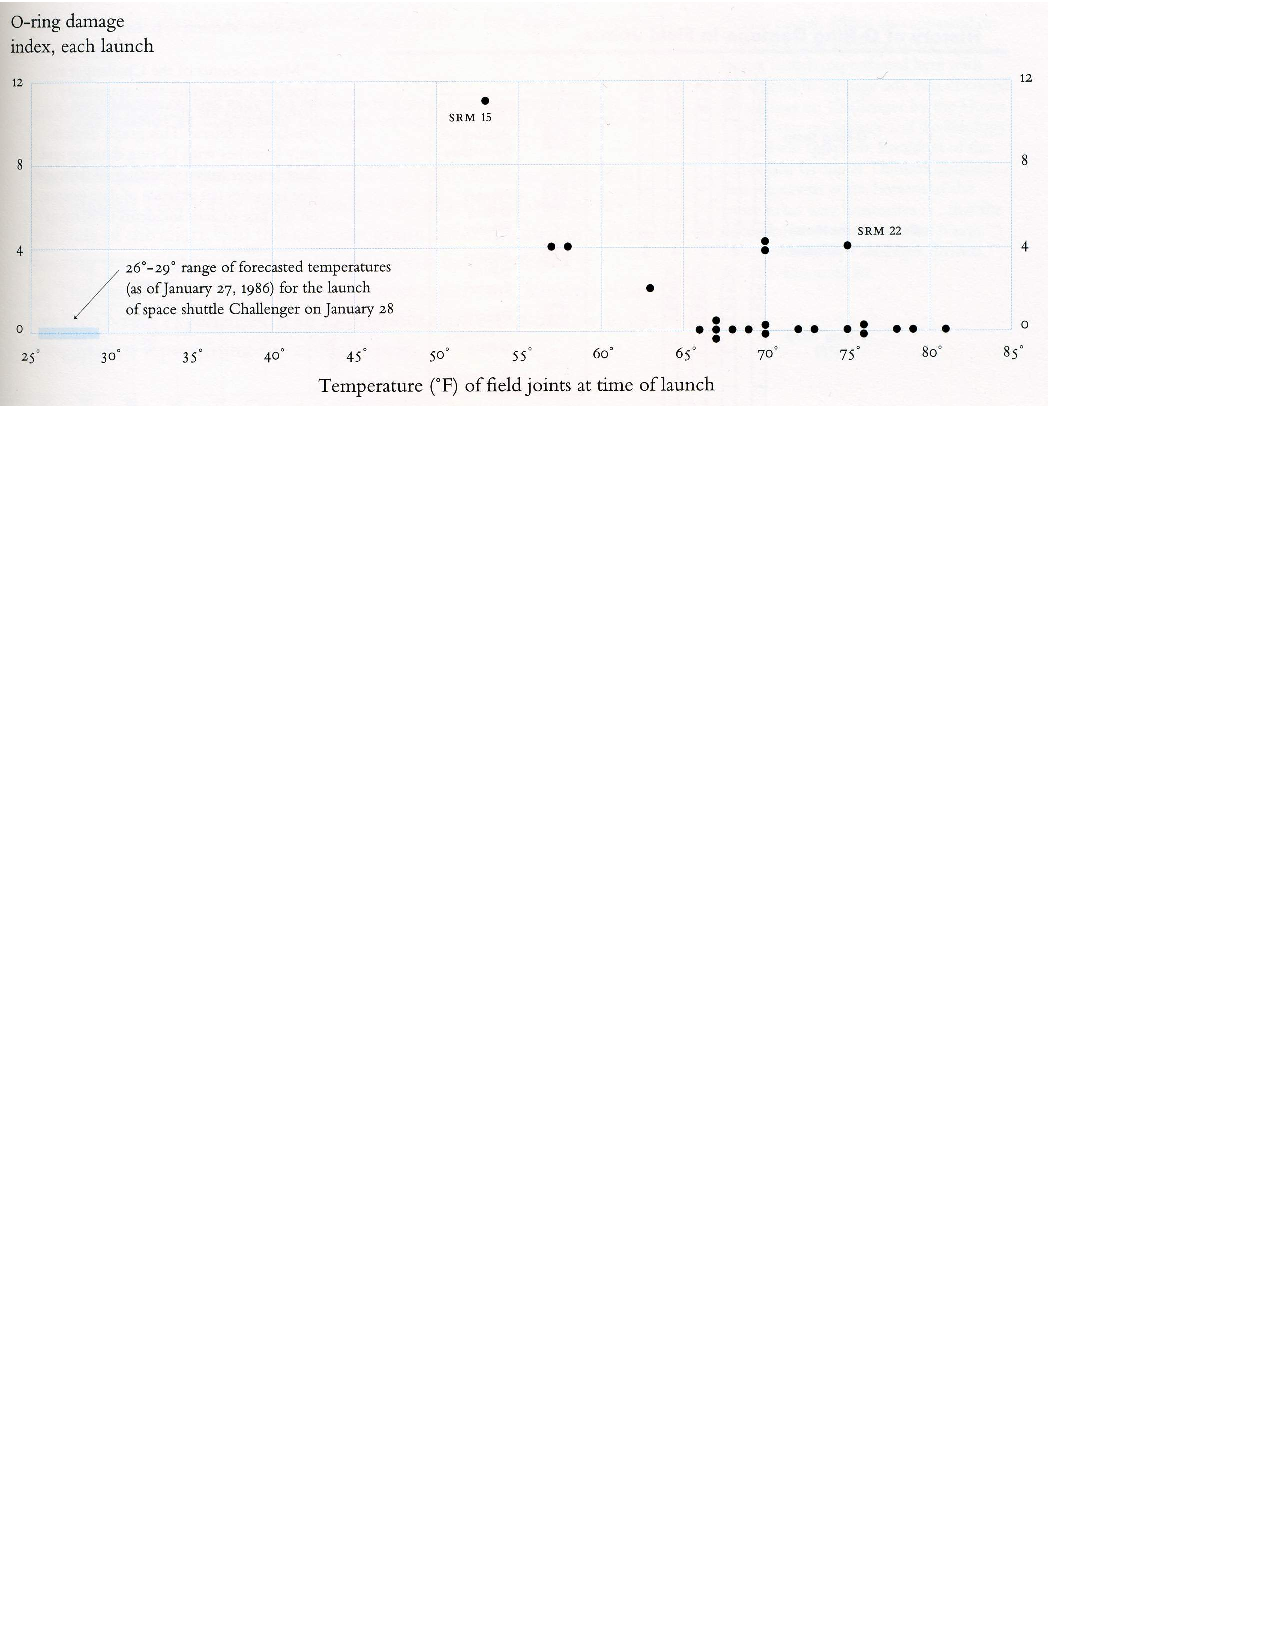
\includegraphics[scale=.65]{tufte_challenger_2}
\end{center}


The shuttle was launched in unprecedented cold
\end{frame}

%%%%%%%%%%%%%%%%%%%%%%%%%%%%%%%%%%%

\begin{frame}{The \textit{Challenger} launch decision}

\small{
Imagine you are the analyst making the launch recommendation.

You've made the scatterplot above.  What would you add to it?

Put another way, what do you is the first question you expect from your boss? \pause

``What's the chance of failure at 26 $^{\circ}$F?'' \pause

The scatterplot suggests the answer is ``high'', but that's vague \pause

But what if the next launch is at 58 $^{\circ}$F?  Or 67 $^{\circ}$F? \pause

Clearly, we want a more precise way to state the probability of failure

We need a \textit{model}, and a way to convey that model to the public.}
\end{frame}

%%%%%%%%%%%%%%%%%%%%%%%%%%%%%%%%%%%

\begin{frame}{The \textit{Challenger} launch decision}

\begin{footnotesize}
Model the probability of O-ring damage as a function of temperature

We can use a statistical tool called ``logit'' for this purpose 

The model is nonlinear: \quad  $\mathrm{Pr(damage)}
  = (1 - \mathrm{exp}(-\beta_0 -\beta_1\mathrm{temperature}))^{-1}$ \pause

\texttt{R} gives us this lovely logit output{\ldots} \pause

\scriptsize{
\begin{center}
\begin{tabular}{llll}
\toprule
Variable  &   \multicolumn{1}{c}{est.}   &   \multicolumn{1}{c}{s.e.}   &  \multicolumn{1}{c}{$p$} \\
\midrule
Temperature (F)  &  -0.18 &  0.09  & 0.047 \\
Constant     &  11.9&  6.34 &  0.062 \\
\midrule
$N$            &  22 & & \\
log-likelihood & -10.9 & & \\
\bottomrule
\end{tabular}
\end{center}
}
which most social scientists read as ``a statistically significant negative relationship b/w temperature and probability of damage''

But that's pretty vague too.

Is there a more persuasive/clear/useful way to present these results?
\end{footnotesize}

\end{frame}

%%%%%%%%%%%%%%%%%%%%%%%%%%%%%%%%%%%

\begin{frame}
\begin{center}
\includegraphics<1>[scale=.8]{chall1}
\includegraphics<2>[scale=.8]{chall2}
\includegraphics<3>[scale=.8]{chall3}
\includegraphics<4>[scale=.8]{chall4}
\includegraphics<5>[scale=.8]{chall5}
\includegraphics<6>[scale=.8]{chall6}

\end{center}

\scriptsize{
\only<1>{A picture clearly shows non-linear model predictions \emph{and} uncertainty}

\only<2>{And gives a more precise sense of how foolhardy launching at 29 F is.}

\only<3>{It's also good to show the data giving rise to the model.
}

\only<4>{Remembering that the Failures are only meaningful compared to Successes}

\only<5>{Looking just at the data might show that launches under 66 F likely O-ring failures.}

\only<6>{This inference is based on an unstated model.}
}
\end{frame}

%%%%%%%%%%%%%%%%%%%%%%%%%%%%%%%%%%%

\begin{frame}


\begin{center}
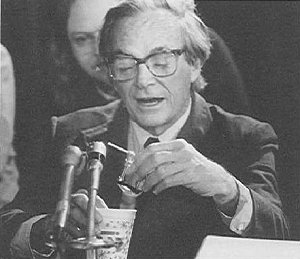
\includegraphics[scale=.6]{feynnman.jpg}
\end{center}
\begin{footnotesize}

In a hearing, Richard Feynmann dramatically showed O-rings lose resilence when cold by dropping one in his ice water.

Experiment cut thru weeks of technical gibberish concealing flaws in the O-ring

But it shouldn't have taken a Nobel laureate: \\ 
any scientist with a year of statistical training could have used the launch record to reach the same conclusion

And it would take no more than a single graphic to show the result
\end{footnotesize}

\end{frame}

%%%%%%%%%%%%%%%%%%%%%%%%%%%%%%%%%%%

\end{document}

%%%%%%%%%%%%%%%%%%%%%%%%%%%%%%%%%%%